\chapter{Beginning Algebra}

\section{Intro}

This course covers 9th grade math, i.e. the first year of high school mathematics.

\section{The Three Forms of Linear Equations and Finding Slope}

% \vspace{1 cm}

% \centerline{\textbf{\large The Slope of a Line}}

% \vspace{0.2 cm}

If \(A(x_{1},y_{1})\text{ and } B(x_{2},y_{2})\) are two points on a line, \textbf{the slope of the line} is defined by the equation below.

\begin{equation}
  m = \frac{y_{2}-y_{1}}{x_{2}-x_{1}}
  \label{eq:3.1}
\end{equation}

\hl{Slope} (hệ số góc) measures the steepness of a line. If the slope of a line is positive, the line travels up moving from left to right. If the slope of a line is negative, the line travels down moving left to right. If the slope of a line is zero, the line is horizontal. If the slope of a line is undefined, the line is vertical.

\textbf{Slope} (hệ số góc) cho biết rate of change. Two parallel lines have \textit{the same} slope.

\begin{figure}[htb!]
  \centering
  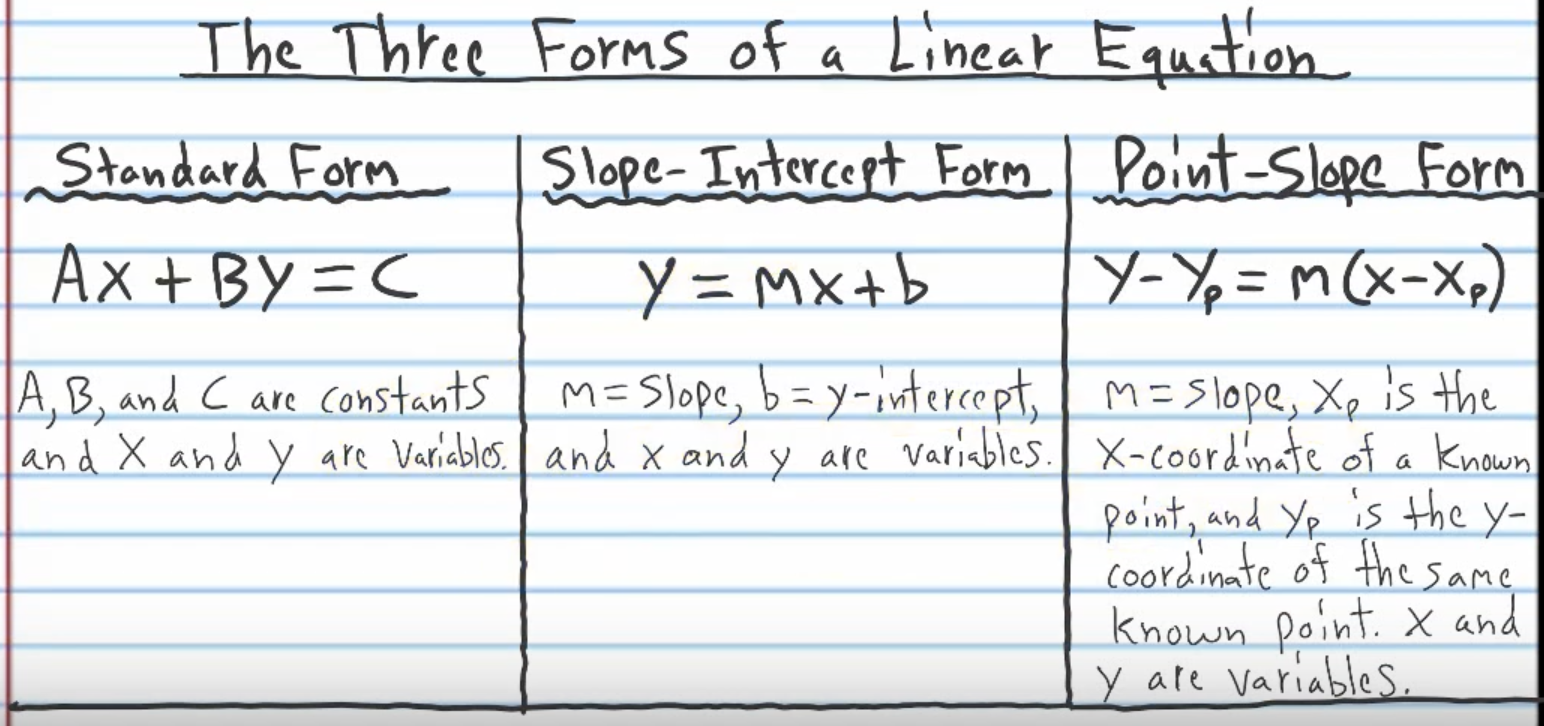
\includegraphics[width=1\textwidth]{beg2601.png}
  \caption{The Three Forms of a Linear Equation}
\end{figure}

% \par\rule{\textwidth}{0.5pt}

\textbf{Excercise}: Identify the form of each linear equation below by writing \q{S} for Standard, \q{SI} for slope-intercept, or \q{PS} for point-slope.

$2x+4y=3$: \textbf{S} because the variables x and y are on the same side of the equation.

$4=-8x+7x$: still Standard form, even though the equation is flipped.

$y-4=-3(x-5)$: \textbf{PS}, it is the only form that has parenthesses.

$y=2x+4$: \textbf{SI}, because the y is isolated on one side of the equation.

\par\rule{\textwidth}{0.5pt}

\textbf{Q:} Graph this line \(3x-4y=-6\)

Find the \textbf{x-intercept} by making y = 0. Then find the \textbf{y-intercept} by making x = 0.

\vspace{5mm}

\textbf{Q:} Graph this inequality \(y < -\frac{1}{3}x+2\)

Tìm tọa độ 2 điểm; vẽ đường thẳng.

\begin{itemize}
  \item Nếu \(\le\) thì vẽ straight line and shade under the line.
  \item Nếu > thì vẽ dashed line and shade above the line.
\end{itemize}

\textbf{Q: }Graphing Systems of Inequalities

\vspace{5mm}

Tính \textbf{Distance between 2 points} bằng Eq \ref{eq:3.2} below:

\begin{equation}
  d = \sqrt{(x_{1}-x_{2})^{2} + (y_{1}-y_{2})^{2}}
  \label{eq:3.2}
\end{equation}

